% Page 9
\thispagestyle{empty} % Supprimer l'en-tête et le pied de page
\begin{center}
    \section{\huge\textbf{{ANNEXES}}}
\end{center}

% Sommaire des figures
\phantomsection % Pour que le lien hypertexte pointe au bon endroit
\renewcommand{\listfigurename}{Sommaire des figures} % Nom du sommaire des figures en français
\listoffigures % Sommaire des figures
\addcontentsline{toc}{section}{Sommaire des annexes} % Ajouter au sommaire général

% Sommaire des tables
\phantomsection % Pour que le lien hypertexte pointe au bon endroit
\renewcommand{\listtablename}{Sommaire des tableaux} % Nom du sommaire des tables en français
\listoftables % Sommaire des tables
\clearpage

% Image 1 ZED2 nuage precision
\begin{figure}[h]
    \centering
    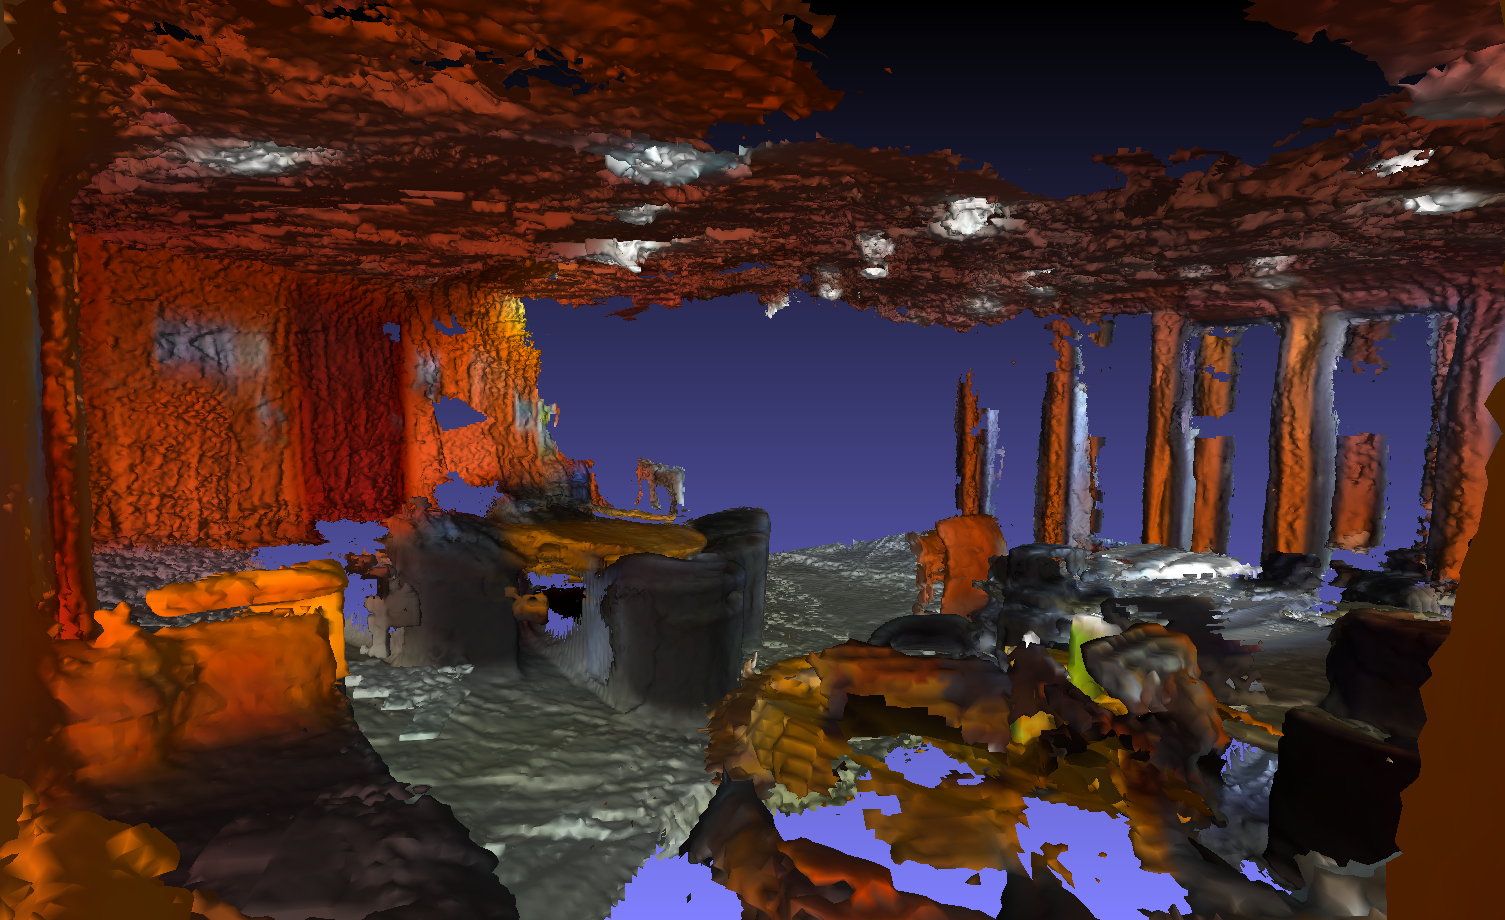
\includegraphics[width=10.5cm]{images/zed2_nuage_colore_2.png}
    \caption{Nuage de points coloré capturé à l'école des Mines de Nancy}
    \label{fig:zed2_1}
\end{figure}

% Image 2 ZED2 nuage coloré
\begin{figure}[h]
    \centering
    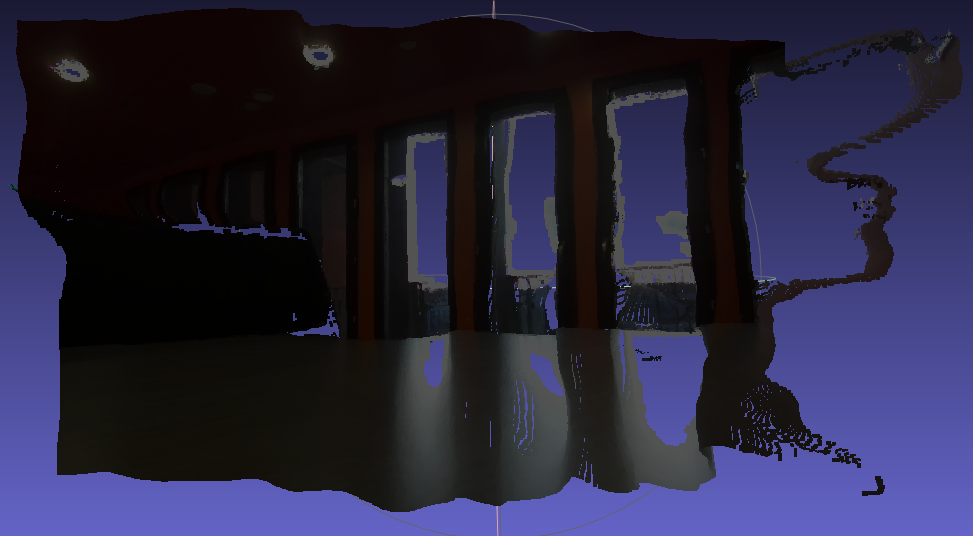
\includegraphics[width=10.5cm]{images/zed2_nuage_colore.png}
    \caption{Nuage de points coloré capturé à l'école des Mines de Nancy}
    \label{fig:zed2_2}
\end{figure}

% Image 1 kinect nuage precision
\begin{figure}[h]
    \centering
    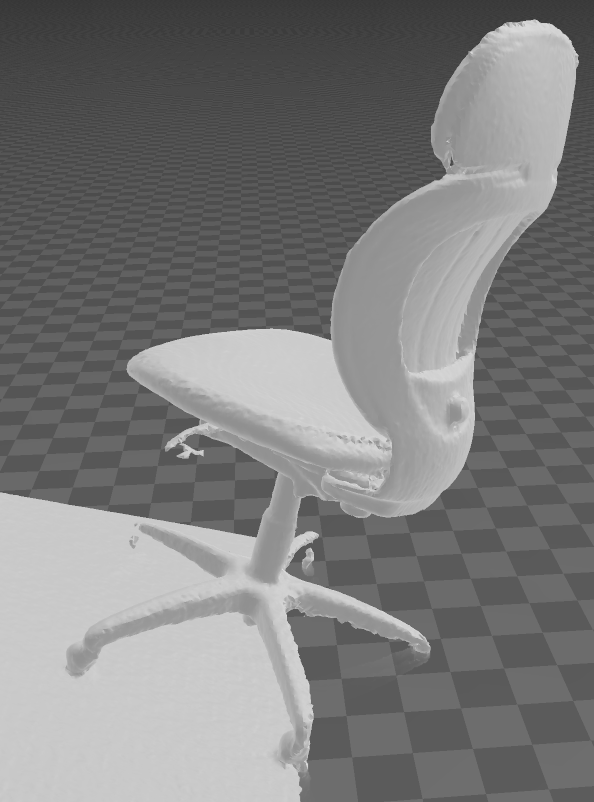
\includegraphics[width=15cm]{images/kinect_sans_couleur.png}
    \caption{Nuage de points brut d'une chaise}
    \label{fig:kinect_1}
\end{figure}


% Image 2 kinect nuage coloré
\begin{figure}[ht]
    \centering
    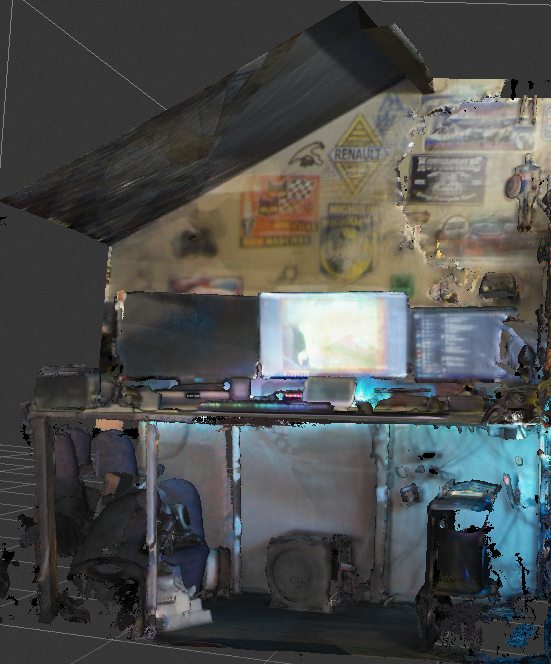
\includegraphics[width=15cm]{images/kinect_avec_couleur.png}
    \caption{Nuage de points coloré d'un bureau}
    \label{fig:kinect_2}
\end{figure}

% Image 1 lidar
\begin{figure}[h]
    \centering
    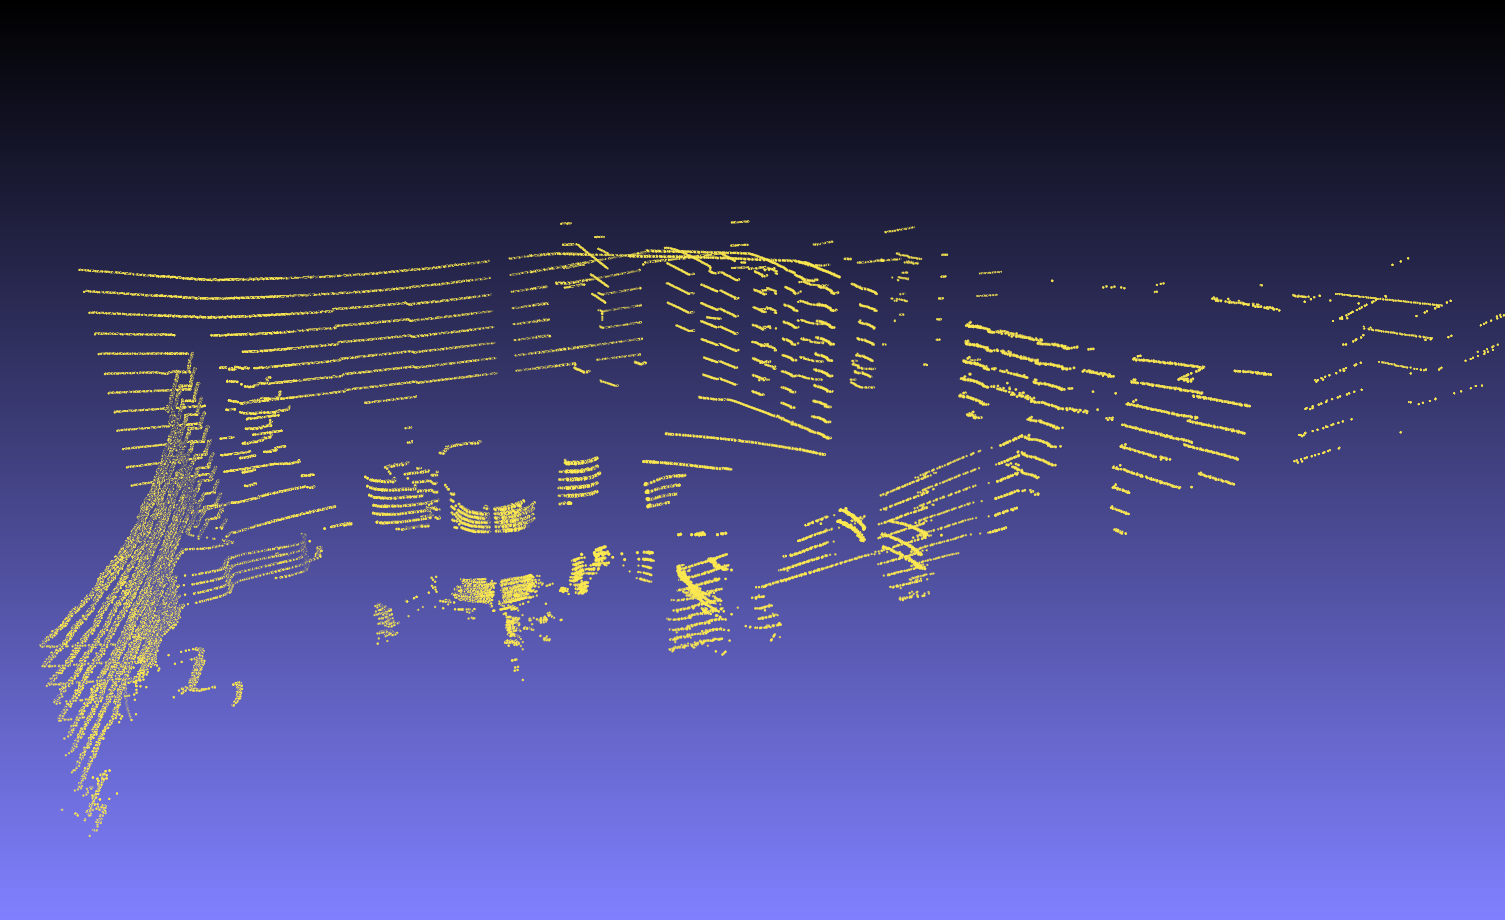
\includegraphics[width=15cm]{images/lidar.png}
    \caption{Nuage de points capturé à l'école des Mines de Nancy}
    \label{fig:lidar}
\end{figure}

\begin{table}[h]
    \centering
    \caption{Comparaison entre ZED 2 / Kinect V1 / Puck Lite}
    \label{tab:comparison}
    \begin{tabularx}{\textwidth}{|>{\hsize=0.6\hsize}X|>{\hsize=0.8\hsize}X|>{\hsize=0.8\hsize}X|>{\hsize=0.8\hsize}X|}
    \hline
    \textbf{Caractéristique} & \textbf{ZED 2} & \textbf{Kinect V1} & \textbf{Puck Lite} \\ \hline
    \textbf{Capture vidéo}    
        & \begin{tabular}[t]{@{}p{1\linewidth}@{}}
            - 2.2K à 15 FPS \\
            - 1080p à 30 FPS \\
            - 720p à 60 FPS \\
            - 376p à 100 FPS
          \end{tabular}
        & \begin{tabular}[t]{@{}p{1\linewidth}@{}}
            - 480p à 30 FPS \\
            - 240p à 30 FPS
          \end{tabular}
        & \cellcolor{lightgray}
        \\ \hline
    \textbf{Vitesse de capture de points} 
        & - 100 Hz 
        & - 30 Hz 
        & \begin{tabular}[t]{@{}p{1\linewidth}@{}} 
          - 300 kHz : en simple \\
          - 600 kHz : en double
          \end{tabular}
        \\ \hline
    \textbf{Vitesse de capture de mouvement} 
        & - 400 Hz 
        & - 30 Hz 
        & \cellcolor{lightgray}
        \\ \hline
    \textbf{Vitesse de capture infrarouge} 
        & \cellcolor{lightgray}
        & - 30 Hz
        & \cellcolor{lightgray}
        \\ \hline 
    \textbf{Densité des nuages} 
        & \cellcolor{lightgray}
        & \cellcolor{lightgray}
        & \begin{tabular}[t]{@{}p{1\linewidth}@{}}
            - $\pm$ 130 pts/mm² à 5 m
          \end{tabular}
        \\ \hline
    \textbf{Précision des points} 
        & $\pm$ 100 mm à 5 m
        & $\pm$ 100 mm à 5 m
        & \begin{tabular}[t]{@{}p{1\linewidth}@{}}
          $\Rightarrow$ $\pm$ 1 mm à 5 m \\
          $\Uparrow$ $\pm$ 3 mm à 5 m
          \end{tabular}
        \\ \hline
    \textbf{Temps de post-traitement}  
        & \begin{tabular}[t]{@{}p{0.8\linewidth}@{}} % 1 => cellule complete 
            De quelques secondes à quelques minutes selon la qualité choisie.
          \end{tabular}
        & \begin{tabular}[t]{@{}p{0.8\linewidth}@{}}
            De quelques secondes à quelques minutes selon la qualité choisie.
          \end{tabular}
        & \begin{tabular}[t]{@{}p{1\linewidth}@{}}
            Quelques secondes.
          \end{tabular}
        \\ \hline
    \textbf{Champ d'action}    
        & \begin{tabular}[t]{@{}p{1\linewidth}@{}}
            $\pm$ 1 m à $\pm$ 20 m
          \end{tabular}
        & \begin{tabular}[t]{@{}p{1\linewidth}@{}}
            $\pm$ 0.8 m à $\pm$ 4 m
          \end{tabular}
        & \begin{tabular}[t]{@{}p{1\linewidth}@{}}
            $\pm$ 0.9 m à $\pm$ 100 m
          \end{tabular}
        \\ \hline
    \textbf{Infos récupérées} 
        & \begin{tabular}[t]{@{}p{0.8\linewidth}@{}}
            - Image RGB x2 \\
            - Nuage de point \\
            - Accéléromètre \\
            - Gyroscope \\
            - Baromètre \\
            - Magnétomètre \\
            - Température
          \end{tabular}
        & \begin{tabular}[t]{@{}p{0.8\linewidth}@{}}
            - Image RGB \\
            - Nuage de point \\
            - Mouvement des objets de son champ de vision \\
            - Microphone
          \end{tabular}
        & \begin{tabular}[t]{@{}p{0.8\linewidth}@{}}
            - Nuage de point \\
            - Mesure de réfléxion \\
            - Angle de rotation \\
            - Horodotage synchronisé \\
            - Position GPS (avec un module en option)
          \end{tabular} 
        \\ \hline
    \textbf{Accès ouvert aux données} 
        & \begin{tabular}[t]{@{}p{0.8\linewidth}@{}} 
          Oui, il existe l'API ZED SDK ainsi que des logiciels.
          \end{tabular}
        & \begin{tabular}[t]{@{}p{0.8\linewidth}@{}} 
          Oui, il existe un kit de développement et un SDK. \\
          Des logiciels tiers sont disponibles comme Skanect ou encore Libfreenect.
          \end{tabular}
        & \begin{tabular}[t]{@{}p{0.8\linewidth}@{}}
            Oui, il existe l'API Paraview ainsi que le logiciel LidarView par exemple.
          \end{tabular}
        \\ \hline
    \end{tabularx}
\end{table}

\clearpage